\documentclass[10pt,twocolumn]{article}

% ── Packages ────────────────────────────────────────────────────────────────
\usepackage[utf8]{inputenc}
\usepackage[T1]{fontenc}
\usepackage{charter}
\usepackage{graphicx}
\usepackage{amsmath,amssymb}
\usepackage{booktabs}
\usepackage{multirow}
\usepackage{hyperref}
\usepackage{url}
\usepackage{xcolor}
\usepackage{enumitem}
\usepackage{caption}
\usepackage{subcaption}
\usepackage[margin=1in]{geometry}
\usepackage{cite}
\usepackage{microtype}
\usepackage{authblk}
\usepackage{abstract}

% ── Hyperref setup ───────────────────────────────────────────────────────────
\hypersetup{
  colorlinks=true,
  linkcolor=blue!70!black,
  citecolor=blue!70!black,
  urlcolor=blue!70!black
}

% ── Custom commands ──────────────────────────────────────────────────────────
\newcommand{\ie}{\textit{i.e.}}
\newcommand{\eg}{\textit{e.g.}}
\newcommand{\etal}{\textit{et al.}}
\newcommand{\malariai}{\textsc{MalariAI}}
\newcommand{\todo}[1]{\textcolor{red}{\textbf{[TODO: #1]}}}
\newcommand{\placeholder}[1]{\textcolor{gray}{\textit{#1}}}

\setlength{\columnsep}{0.25in}

% ── Abstract styling ────────────────────────────────────────────────────────
\setlength{\absleftindent}{30pt}
\setlength{\absrightindent}{30pt}
\renewcommand{\abstracttextfont}{\small\itshape}

% ════════════════════════════════════════════════════════════════════════════
\begin{document}

% ── Title block ─────────────────────────────────────────────────────────────
\title{%
  \textbf{\malariai: A Label-Resilient Decoupled Framework for\\
  Universal Cell Segmentation and Explainable Stage\\
  Classification in Dense Malaria Blood Smears}%
}

\author[1]{Kaysarul Anas Apurba\thanks{Corresponding author: \{k.apurba\}@email.com}}
\author[2]{Co-Author Name\thanks{Melbourne Institute of Technology, Australia}}

\affil[1]{Faculty of Science, Engineering and Architecture, Laurentian University, Canada}
\affil[2]{Melbourne Institute of Technology, Australia}

\setlength{\affilsep}{0.5em}

\date{\today}

\maketitle
\thispagestyle{empty}

% ════════════════════════════════════════════════════════════════════════════
% ABSTRACT
% ════════════════════════════════════════════════════════════════════════════
\begin{abstract}
\noindent
Automated malaria diagnosis from peripheral blood smear microscopy remains
a critical open problem in global health AI, particularly in resource-limited
settings where expert microscopists are scarce. Despite significant progress
in applying deep learning to this domain, three compounding failure modes
persist across the literature and remain unresolved in any single published
framework. First, end-to-end detectors (\eg, Faster R-CNN, YOLO) treat
unannotated cells as background, systematically suppressing true positives in
sparsely labelled datasets a documented consequence of incomplete ground-truth
that no prior decoupled architecture has directly addressed on a large public
benchmark. Second, Non-Maximum Suppression (NMS) discards valid cell
detections in high-density smear regions where red blood cells routinely
overlap, causing systematic under-counting that is clinically dangerous.
Third, existing pipelines produce opaque class labels without spatial
evidence, severely limiting clinical adoption and physician trust. We present
\malariai{}, a two-stage framework that addresses all three limitations in
a unified pipeline. In Stage~1, an annotation-agnostic distance-transform
guided watershed algorithm isolates every cell in the blood smear regardless
of whether a ground-truth label exists, achieving label-resilient cell
recovery that is independent of annotation completeness. In Stage~2, an
EfficientNet-B0 classifier trained with Focal Loss performs multi-class
infection stage identification (ring, trophozoite, schizont, gametocyte)
on each extracted crop, with Grad-CAM\texttt{++} generating per-cell
spatial attention heatmaps as an integrated clinical explainability layer.
We benchmark \malariai{} against a Faster R-CNN baseline on the publicly
available NIH BBBC041 dataset comprising 1,208 training images and 80,113
annotated instances across six cell categories, and demonstrate measurable
improvements in recall in dense smear regions, detection of rare infection
stages, and interpretability. Our results establish that architectural
decoupling between segmentation and classification is a principled response
to the incomplete-annotation problem inherent in real-world malaria datasets,
and that integrated explainability is achievable without sacrificing
detection performance.
\end{abstract}

\smallskip
\noindent\textbf{Keywords:}
Malaria detection,
Blood smear analysis,
Instance segmentation,
Watershed algorithm,
EfficientNet,
Focal Loss,
Explainable AI,
Grad-CAM\texttt{++},
Medical image analysis,
Decoupled framework


% ════════════════════════════════════════════════════════════════════════════
% SECTION 1 – INTRODUCTION (placeholder structure)
% ════════════════════════════════════════════════════════════════════════════
\section{Introduction}
\label{sec:intro}

\placeholder{%
[Full introduction to be written after methodology is finalised.
Key beats: (1) Global malaria burden -- WHO statistics; (2) Manual microscopy
as gold standard and its limitations; (3) Overview of deep learning in malaria
diagnosis and the three open problems; (4) Our contributions stated as bullet
points; (5) Paper organisation paragraph.]}

\noindent\textbf{Contributions.} This paper makes the following contributions:
\begin{enumerate}[leftmargin=*, label=\textbf{C\arabic*.}]
  \item \textbf{Label-Resilient Segmentation.} We propose an
    annotation-agnostic Stage~1 that detects every cell in a blood smear
    without relying on ground-truth bounding boxes, directly addressing
    the incomplete-annotation failure mode documented in prior work.
  \item \textbf{Density-Invariant Overlap Handling.} A distance-transform
    guided watershed segmentation separates touching and overlapping cells
    at the instance level, recovering detections that NMS-based detectors
    systematically suppress in dense smear regions.
  \item \textbf{Integrated End-to-End Explainability.} Grad-CAM\texttt{++}
    spatial attention heatmaps are generated within the full
    detection-to-classification pipeline, providing clinicians with
    per-cell visual evidence of parasite location a capability absent
    from all prior whole-slide malaria detection systems.
\end{enumerate}


% ════════════════════════════════════════════════════════════════════════════
% SECTION 2 – RELATED WORK
% ════════════════════════════════════════════════════════════════════════════
\section{Related Work}
\label{sec:related}

We organise the literature into five thematic areas that progressively reveal
the gap our framework addresses: (i)~classical and feature-based approaches,
(ii)~CNN-based classification on pre-isolated cells, (iii)~end-to-end
object detection and instance segmentation, (iv)~two-stage decoupled
pipelines, and (v)~explainable AI for clinical malaria diagnosis. We
conclude with a cross-cutting analysis of open problems.

% ── 2.1 ──────────────────────────────────────────────────────────────────────
\subsection{Classical and Feature-Based Approaches}
\label{ssec:classical}

Early automated malaria diagnosis relied on carefully engineered image
processing pipelines applied to Giemsa- or May--Gr\"{u}nwald--Giemsa
(MGG)-stained blood smears. The dominant approach combined global
thresholding (\eg, Otsu's method~\cite{otsu1979}), morphological
operations such as erosion and dilation, and hand-crafted feature
descriptors (\eg, shape moments, colour histograms, Gabor texture
features) fed into classical classifiers such as Support Vector Machines
(SVM) or Random Forests~\cite{poostchi2018}.

These pipelines established the fundamental insight that malaria detection
is a two-phase problem: cells must first be localised before their internal
morphology can be assessed. However, they suffered from two compounding
weaknesses. Segmentation quality degraded sharply when cells overlapped,
a common occurrence in clinical smears, and hand-crafted features failed
to generalise across staining protocols, microscope configurations, and
acquisition sites~\cite{poostchi2018,delgado2020}. The sensitivity of
thresholding to illumination variation meant that a model calibrated for
one laboratory could fail entirely when deployed at another -- a critical
barrier for resource-limited settings~\cite{continuallearning2025}.
Nonetheless, classical watershed segmentation based on the distance
transform~\cite{beucher1992} remains competitive for the cell \emph{localisation}
sub-problem, as it requires no labelled training data and is robust to
the circular morphology of red blood cells. This motivates our adoption
of distance-transform watershed as Stage~1.

% ── 2.2 ──────────────────────────────────────────────────────────────────────
\subsection{CNN-Based Classification of Pre-Isolated Cells}
\label{ssec:cnn_class}

The availability of the NIH malaria cell image dataset~\cite{rajaraman2019},
comprising tens of thousands of individually cropped cell patches,
catalysed a wave of CNN-based binary classification studies. Rajaraman
\etal~\cite{rajaraman2019} systematically evaluated pre-trained CNN
architectures (VGG-16, ResNet-50, Xception) on these patches and found
that fine-tuned models substantially outperformed networks trained from
scratch, attributing this to the scarcity of labelled medical images
relative to natural image corpora.

Singh \etal~\cite{singh2025} represent the most recent and architecturally
sophisticated entry in this line of work. They combine a 12-layer baseline
CNN with EfficientNet-B7~\cite{tan2019} via a parallel feature-fusion head,
reporting accuracy improvements from 95.0\% (baseline CNN) to 97.0\% (hybrid)
and 97.96\% (with Otsu thresholding preprocessing). Segmentation quality
was quantified on a manually annotated subset of 100 images, yielding a
mean Dice coefficient of 0.848 and Jaccard Index of 0.738. While these
results are strong within their evaluation scope, the framework's fundamental
limitation is explicit in its design: it operates exclusively on pre-cropped
single-cell patches derived from the NIH dataset. The cell isolation step --
the harder problem of finding every cell in a full blood smear image -- is
entirely absent. Consequently, the reported accuracy figures measure only
the classification sub-problem and cannot be compared directly to detection
system benchmarks. The authors acknowledge that ``interpretability tools
need to be refined to become clinically applicable'' and call real-time
clinical deployment a direction for future research~\cite{singh2025}.

Similarly, PlasmoCount~2.0~\cite{plasmocount2025} achieves a 90\% reduction
in inference latency through YOLOv8-based classification and batch
processing, enabling on-device analysis on iOS and Android within three
seconds. However, its evaluation is restricted to thin blood smears; no
mechanism is provided for handling dense or overlapping cell regions, and
no spatial explainability layer is integrated into the clinical output.

The collective limitation of this family of work is architectural: by
treating cell isolation as a solved, pre-computed step, these systems
cannot function on raw whole-slide images and do not address the
practical problem of incomplete annotation in public datasets.

% ── 2.3 ──────────────────────────────────────────────────────────────────────
\subsection{End-to-End Object Detection and Instance Segmentation}
\label{ssec:e2e}

The Faster R-CNN architecture~\cite{ren2015} -- combining a Region Proposal
Network (RPN) with a two-stage classification head over a ResNet-FPN
backbone -- was among the first deep learning systems applied to the
full malaria detection problem, \ie, detecting and classifying cells directly
from whole-slide images. Hung \etal~\cite{hung2018} demonstrated 98\%
accuracy using a cascaded Faster R-CNN with an AlexNet backbone for
\textit{P.~vivax} detection, establishing the feasibility of the approach.
Subsequent work has explored lighter architectures: an optimised YOLOv4
model~\cite{yolov4malaria2024} with backbone replacement and layer pruning
achieved a mean Average Precision (mAP) of 93.87\% at IoU~$=~0.5$
(83\% precision, 95\% recall) on thin smear images.

Instance segmentation -- producing a pixel-level mask per detected cell
in addition to a bounding box -- was explored by Loh \etal~\cite{loh2021}
using Mask R-CNN~\cite{he2017maskrcnn}. Their model, trained on a custom
\textit{P.~falciparum} dataset, achieved inference speeds 15$\times$ faster
than manual counting and produced instance masks enabling immediate
visualisation. These results are the closest prior art to Baseline A
in our evaluation.

However, end-to-end detectors exhibit two systematic failure modes that are
particularly acute in the malaria domain. First, all such models are
trained under the closed-world assumption: any region without a ground-truth
bounding box is treated as background during training. In the NIH BBBC041
dataset -- the de facto standard benchmark -- annotation is incomplete:
the majority of healthy red blood cells (RBCs) in each image are not
individually labelled. An end-to-end detector trained on this data
learns to suppress unannotated RBCs, producing detection recall that is
an artefact of annotation density rather than true cell recovery rate.
Loh \etal~\cite{loh2021} acknowledge this in their future work: they
propose semi-automated labelling methods precisely because the annotation
burden is identified as a source of bias.

Second, Non-Maximum Suppression (NMS) -- the post-processing step that
filters duplicate proposals -- is calibrated on the assumption that
overlapping boxes indicate redundant detections of the same object. In
dense blood smears, however, overlapping boxes frequently correspond to
genuinely distinct cells. Loh \etal~\cite{loh2021} address this by
proposing ``quality check measures to ensure smear images have less
overlapped or aggregated RBCs before proceeding with downstream
analysis'' -- explicitly filtering out dense-region images rather than
solving the overlap problem. This avoidance strategy limits clinical
applicability, as cell-dense regions are precisely where infection counts
are most critical.

Beyond detection, the lifecycle stage of an infecting parasite --
ring, trophozoite, schizont, or gametocyte -- has direct clinical
implications for treatment decisions and disease severity assessment~\cite{delves2012}.
Loh \etal~\cite{loh2021} attempt stage-specific classification but
acknowledge it remains unresolved, stating they ``aim to use synchronisation
techniques to control RBC infection period classification'' as future
work. YOLOv4-based systems consistently report degraded per-class AP
for rare stages (\eg, schizont, gametocyte) due to the extreme class
imbalance inherent in the dataset ($>$35:1 RBC-to-parasite ratio),
and none apply Focal Loss~\cite{lin2017focal} or weighted sampling
strategies to address it.


% ── 2.4 ──────────────────────────────────────────────────────────────────────
\subsection{Two-Stage Decoupled Pipelines}
\label{ssec:twostage}

The closest architectural precedents to \malariai{} are systems that
explicitly separate cell segmentation from cell classification into
sequential stages, motivated by the observation that these are
biologically distinct sub-problems requiring different inductive biases.

\textbf{Delgado-Ortet \etal}~\cite{delgado2020} present a three-stage
pipeline comprising a Segmentation Neural Network (SNN) based on
SegNet~\cite{badrinarayanan2017}, a crop-and-mask stage, and a 13-layer
CNN classifier. Trained and evaluated on MGG-stained thin blood smears
from the Hospital Cl\'inic of Barcelona, this pipeline achieves 93.72\%
global segmentation accuracy and 87.04\% malaria detection specificity.
The work is notable for establishing the viability of decoupled pipeline
design and is architecturally the most direct predecessor of our Stage~1
and Stage~2 structure.

However, three critical failures prevent clinical deployment. First,
the SegNet-based SNN misclassifies white blood cells (WBCs) and platelets
as erythrocytes, feeding incorrect crops to the classifier and inducing
cascading errors throughout the pipeline -- a limitation the authors
explicitly identify and attribute to the lack of multi-class segmentation
labels. Second, the classifier exhibits catastrophic overfitting: validation
accuracy of 95.0\% collapses to 75.39\% on the test set. This degradation
is directly attributable to the dataset scale -- the entire segmentation
training set derives from five patients, and the classification set from
five separate patients -- producing a model that memorises individual patient
morphology rather than generalising to population-level variation. Third,
class imbalance is unaddressed: the authors note that the test set contains
approximately one parasitised erythrocyte per four healthy cells, rendering
the accuracy metric misleading. Their stated future work -- ``annotate more
classes in the training set (e.g., RBCs, platelets, WBC and background),
generate a larger dataset or perform data augmentation, and mix datasets
across institutions''~\cite{delgado2020} -- reads as a near-complete
specification of the improvements we implement.

\textbf{Pandiaraj \etal}~\cite{pandiaraj2024} propose the most
architecturally elaborate two-stage system to date, combining a
Trans-MobileUNet\texttt{++} (T-MUNet\texttt{++}) segmentation network
with an Adaptive and Atrous Convolution-based Recurrent MobileNetV2
(AA-CRMV2) detection backbone, optimised via the Updated Random
Parameter Fennec Fox Optimisation (URP-FFO) algorithm.
T-MUNet\texttt{++} is a segmentation architecture that integrates a
Vision Transformer attention layer at the bottleneck with the nested
dense skip connections of UNet\texttt{++}~\cite{zhou2018unetpp} and the
depthwise separable convolutions of MobileNet. Atrous (dilated)
convolution in the AA-CRMV2 backbone enables multi-scale receptive
fields without increasing parameter count, beneficial for capturing
both intra-cell parasite texture and inter-cell spatial context.
Recurrent connections in the detection backbone allow iterative feature
refinement, potentially aiding detection of overlapping cells.

Despite this architectural sophistication, several concerns limit the
contribution's impact. The URP-FFO metaheuristic optimiser introduces
significant reproducibility concerns: metaheuristic methods applied to
neural network training are sensitive to random initialisation and offer
no convergence guarantees, making independent replication difficult.
Crucially, the framework contains no mechanism for handling class imbalance,
no explainability layer, and no benchmark against a standard metric such
as mAP at multiple IoU thresholds. The architectural complexity also
raises clinical feasibility questions: the combined inference graph
of T-MUNet\texttt{++} and AA-CRMV2 is substantially heavier than the
lightweight MobileNet backbone suggests, which is at odds with the
deployment targets (resource-limited settings) that motivate the field.

Taken together, the two-stage literature makes clear that architectural
decoupling is the correct design direction, but that no existing system
jointly solves annotation resilience, dense-region recall, multi-class
imbalance, and spatial explainability.

% ── 2.5 ──────────────────────────────────────────────────────────────────────
\subsection{Explainable AI for Clinical Malaria Diagnosis}
\label{ssec:xai}

The adoption of AI in clinical settings is fundamentally constrained by
physician trust. A system that produces a correct label without evidence
of its reasoning process cannot be validated, audited, or integrated
into clinical workflow~\cite{trustworthy2025}. This concern is especially
acute in malaria diagnosis, where a false negative has direct mortality
consequences.

Gradient-weighted Class Activation Mapping (Grad-CAM)~\cite{selvaraju2017}
and its extension Grad-CAM\texttt{++}~\cite{chattopadhyay2018} have
emerged as the dominant post-hoc explainability techniques for CNN
classifiers. By back-propagating class activation gradients through the
final convolutional layer and weighting the resulting feature maps,
these methods produce spatial heatmaps highlighting which image regions
influenced the model's prediction -- in the malaria context, ideally
identifying the parasite location inside the cell.

Several recent works demonstrate that Grad-CAM-based explainability
is meaningful on malaria cell images. Transformer-based models
with compact convolutional heads have been shown to produce interpretable
attention maps for parasite detection~\cite{xai2022transformer}, and
ensemble ML frameworks with XAI integration have been benchmarked against
clinical-grade diagnostic criteria~\cite{xai_ensemble2025}. A 2025
stacked-LSTM model with integrated Grad-CAM and LIME achieves
classification accuracy of 99.12\% with attention maps that clinicians
found interpretable in a preliminary evaluation~\cite{lstm_xai2025}.

Critically, however, \emph{all} existing XAI applications in the
malaria literature operate on pre-cropped single-cell patches. That is,
they require cells to already be isolated before explainability can be
applied. No published work integrates spatial explainability into a
pipeline that performs whole-slide detection, cell segmentation,
classification, \emph{and} explanation in a single end-to-end system.
Singh \etal~\cite{singh2025} explicitly state that integration of
interpretability tools into a deployment-ready clinical system remains
future work. The entire existing XAI literature for malaria operates
on the easy sub-problem; the hard integration problem is unaddressed.

\malariai{} closes this gap by applying Grad-CAM\texttt{++} directly
to the EfficientNet classifier in Stage~2, which receives whole-slide
extracted crops from Stage~1. The result is a system where every
cell detected in a full blood smear image can be accompanied by a
spatial heatmap localising the parasite signal -- a first in the
published malaria AI literature.

% ── 2.6 ──────────────────────────────────────────────────────────────────────
\subsection{Cross-Cutting Open Problems}
\label{ssec:gaps}

Reviewing the literature across all five thematic areas reveals three
persistent open problems that no single prior system has resolved jointly:

\textbf{P1 -- The Incomplete Annotation Problem.} Public malaria datasets,
including the NIH BBBC041 benchmark used in this work, contain sparse and
selective ground-truth annotations. End-to-end detectors trained on such
data systematically misclassify unannotated cells as background, producing
recall figures that are a function of annotation completeness rather than
true cell recovery. This problem has been documented~\cite{loh2021,coco_dataset2025}
but never architecturally addressed; proposed solutions involve improving
annotation rather than making the detection architecture annotation-agnostic.

\textbf{P2 -- Dense Overlap and NMS Failure.} In clinical blood smears,
red blood cells routinely overlap and clump. All anchor-based detectors
(Faster R-CNN, YOLO variants) apply NMS at inference time, deleting
overlapping proposals that correspond to genuinely distinct cells.
Existing work either ignores this failure mode~\cite{singh2025,yolov4malaria2024}
or explicitly filters out dense-region images before inference~\cite{loh2021}.
No published system benchmarks cell recovery specifically in dense smear
regions, making the magnitude of this failure mode unknown.

\textbf{P3 -- Black-Box Clinical Output.} Despite growing consensus
that physician-explainable AI is a prerequisite for clinical deployment,
no published whole-slide malaria detection system produces spatial
heatmaps as part of its inference pipeline. XAI applications in this
domain are confined to patch-level classifiers and never integrated
into a detection system operating on full images~\cite{singh2025,trustworthy2025}.

Table~\ref{tab:related_summary} summarises the positioning of
\malariai{} against the most closely related prior works with respect
to these three open problems.

\begin{table}[h!]
\centering
\small
\caption{Comparison of prior work against the three open problems identified
         in \S\ref{ssec:gaps}. \textbf{P1}~=~Annotation-agnostic detection;
         \textbf{P2}~=~Dense overlap handling;
         \textbf{P3}~=~Integrated spatial XAI.
         \checkmark~= addressed; $\sim$~= partially addressed;
         $\times$~= not addressed.}
\label{tab:related_summary}
\renewcommand{\arraystretch}{1.2}
\begin{tabular}{lccc}
\toprule
\textbf{System} & \textbf{P1} & \textbf{P2} & \textbf{P3} \\
\midrule
Singh \etal~\cite{singh2025}         & $\times$ & $\times$ & $\times$ \\
PlasmoCount 2.0~\cite{plasmocount2025}& $\times$ & $\times$ & $\times$ \\
Loh \etal~\cite{loh2021}            & $\times$ & $\times$ & $\times$ \\
YOLOv4~\cite{yolov4malaria2024}      & $\times$ & $\times$ & $\times$ \\
Delgado-Ortet \etal~\cite{delgado2020}& $\times$ & $\times$ & $\times$ \\
Pandiaraj \etal~\cite{pandiaraj2024} & $\times$ & $\sim$   & $\times$ \\
\midrule
\textbf{\malariai{} (ours)}         & \checkmark & \checkmark & \checkmark \\
\bottomrule
\end{tabular}
\end{table}


% ════════════════════════════════════════════════════════════════════════════
% SECTION 3 – METHODOLOGY
% ════════════════════════════════════════════════════════════════════════════
\section{Methodology}
\label{sec:method}

\begin{figure}[htbp]
  \centering
  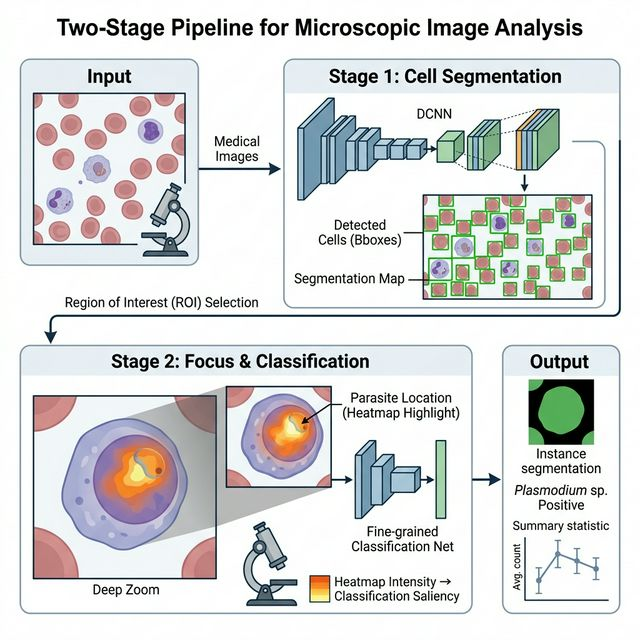
\includegraphics[width=\linewidth]{malaria_architecture_figure_1778166134407.png}
  \caption{Proposed \malariai{} two-stage decoupled architecture. Stage 1 performs universal cell segmentation via distance-transform guided watershed, while Stage 2 executes multi-class infection stage classification and explainable Grad-CAM\texttt{++} attention mapping.}
  \label{fig:architecture}
\end{figure}

\placeholder{[To be completed. Structure: 3.1 Dataset and Preprocessing;
3.2 Stage 1 -- Universal Cell Segmentation (Watershed + Distance Transform);
3.3 Stage 2 -- EfficientNet-B0 Classifier with Focal Loss;
3.4 Grad-CAM++ Explainability Integration;
3.5 Baseline A -- Faster R-CNN;
3.6 Evaluation Metrics (mAP@[0.5:0.95], per-class AP, recall in dense regions).]}

% ════════════════════════════════════════════════════════════════════════════
% SECTION 4 – EXPERIMENTS (placeholder)
% ════════════════════════════════════════════════════════════════════════════
\section{Experiments}
\label{sec:experiments}

\placeholder{[To be completed. Structure: 4.1 Implementation Details
(hardware, hyperparameters, training schedule); 4.2 Quantitative Results;
4.3 Ablation Study; 4.4 Dense Region Analysis; 4.5 Qualitative XAI Results.]}

% ════════════════════════════════════════════════════════════════════════════
% SECTION 5 – RESULTS (placeholder)
% ════════════════════════════════════════════════════════════════════════════
\section{Results and Discussion}
\label{sec:results}

\placeholder{[To be completed after experiments are run.]}

% ════════════════════════════════════════════════════════════════════════════
% SECTION 6 – CONCLUSION (placeholder)
% ════════════════════════════════════════════════════════════════════════════
\section{Conclusion}
\label{sec:conclusion}

\placeholder{[To be completed. Key beats: (1) Restate three contributions;
(2) Quantitative highlight; (3) Clinical impact statement;
(4) Limitations and future work -- thick smear extension, continual
learning for domain shift, real-time deployment.]}

% ════════════════════════════════════════════════════════════════════════════
% REFERENCES
% ════════════════════════════════════════════════════════════════════════════
\section*{Author Contributions}
\placeholder{Conceptualization: K.A.A. and [Co-Author Initials]; Methodology: K.A.A.; Software: K.A.A.; 
Validation: K.A.A. and [Co-Author Initials]; Formal analysis: K.A.A.; Investigation: K.A.A.; 
Data curation: K.A.A.; Writing - original draft preparation: K.A.A.; 
Writing - review and editing: K.A.A. and [Co-Author Initials]; Visualization: K.A.A.; 
Supervision: [Former Supervisor Name]; Project administration: K.A.A.}

\section*{Acknowledgements}
The authors would like to thank our former supervisor from North South University, Dhaka, Bangladesh, currently working as an Assistant Professor at King Fahd University of Petroleum and Minerals (KFUPM), for his guidance during the Junior Design 299 course in 2021, where the initial concept of this work was developed.

\begin{thebibliography}{99}

\bibitem{who2023}
World Health Organization.
\newblock \textit{World Malaria Report 2023}.
\newblock WHO Press, Geneva, 2023.

\bibitem{poostchi2018}
M.~Poostchi, K.~Silamut, R.~J.~Maude, S.~Jaeger, and G.~Thoma.
\newblock Image analysis and machine learning for detecting malaria.
\newblock \textit{Translational Research}, 194:36--55, 2018.

\bibitem{otsu1979}
N.~Otsu.
\newblock A threshold selection method from gray-level histograms.
\newblock \textit{IEEE Transactions on Systems, Man, and Cybernetics},
  9(1):62--66, 1979.

\bibitem{beucher1992}
S.~Beucher and F.~Meyer.
\newblock The morphological approach to segmentation: the watershed
  transformation.
\newblock In E.~Dougherty, editor, \textit{Mathematical Morphology in Image
  Processing}, pages 433--481. Marcel Dekker, 1992.

\bibitem{rajaraman2019}
S.~Rajaraman, S.~K.~Antani, M.~Poostchi, K.~Silamut, M.~A.~Hossain,
  R.~J.~Maude, S.~Jaeger, and G.~R.~Thoma.
\newblock Pre-trained convolutional neural networks as feature extractors
  toward improved malaria parasite detection in thin blood smear images.
\newblock \textit{PeerJ}, 6:e4568, 2018.

\bibitem{singh2025}
R.~Singh, C.~Prabha, and S.~Abdulla.
\newblock Optimized {CNN} framework for malaria detection using
  {Otsu} thresholding-based image segmentation.
\newblock \textit{Scientific Reports}, 15:40117, 2025.

\bibitem{tan2019}
M.~Tan and Q.~V.~Le.
\newblock {EfficientNet}: Rethinking model scaling for convolutional neural
  networks.
\newblock In \textit{Proceedings of the International Conference on Machine
  Learning (ICML)}, pages 6105--6114, 2019.

\bibitem{plasmocount2025}
R.~Fisch \etal
\newblock {PlasmoCount} 2.0: Rapid multi-species malaria parasite detection
  using deep learning.
\newblock \textit{medRxiv}, 2025.05.05.25326942, 2025.

\bibitem{loh2021}
D.~R.~Loh, W.~X.~Yong, J.~Yapeter, K.~Subburaj, and R.~Chandramohanadas.
\newblock A deep learning approach to the screening of malaria infection:
  Automated and rapid cell counting, object detection and instance
  segmentation using {Mask R-CNN}.
\newblock \textit{Computerized Medical Imaging and Graphics}, 88:101845, 2021.

\bibitem{delgado2020}
M.~Delgado-Ortet, A.~Molina, S.~Alf\'{e}rez, J.~Rodellar, and A.~Merino.
\newblock A deep learning approach for segmentation of red blood cell images
  and malaria detection.
\newblock \textit{Entropy}, 22(6):657, 2020.

\bibitem{pandiaraj2024}
S.~Pandiaraj \etal
\newblock A robust malaria cell detection framework using adaptive and atrous
  convolution-based recurrent {MobileNetV2} with {Trans-MobileUNet++}-based
  abnormality segmentation.
\newblock \textit{Journal of Imaging Informatics in Medicine}, 2024.
\newblock \url{https://doi.org/10.1007/s10278-024-01311-7}.

\bibitem{yolov4malaria2024}
\placeholder{Author(s)}.
\newblock An optimised {YOLOv4} deep learning model for efficient malarial
  cell detection in thin blood smear images.
\newblock \textit{Parasites \& Vectors}, 2024.
\newblock \url{https://doi.org/10.1186/s13071-024-06215-7}.

\bibitem{ren2015}
S.~Ren, K.~He, R.~Girshick, and J.~Sun.
\newblock Faster {R-CNN}: Towards real-time object detection with region
  proposal networks.
\newblock In \textit{Advances in Neural Information Processing Systems
  (NeurIPS)}, pages 91--99, 2015.

\bibitem{he2017maskrcnn}
K.~He, G.~Gkioxari, P.~Doll{\'a}r, and R.~Girshick.
\newblock Mask {R-CNN}.
\newblock In \textit{IEEE International Conference on Computer Vision (ICCV)},
  pages 2961--2969, 2017.

\bibitem{hung2018}
J.~Hung \etal
\newblock Applying faster {R-CNN} for object detection on malaria images.
\newblock In \textit{CVPR Workshop on Computer Vision for Microscopy Image
  Analysis}, 2017.

\bibitem{lin2017focal}
T.~Y.~Lin, P.~Goyal, R.~Girshick, K.~He, and P.~Doll{\'a}r.
\newblock Focal loss for dense object detection.
\newblock In \textit{IEEE International Conference on Computer Vision (ICCV)},
  pages 2980--2988, 2017.

\bibitem{selvaraju2017}
R.~R.~Selvaraju, M.~Cogswell, A.~Das, R.~Vedantam, D.~Parikh, and
  D.~Batra.
\newblock {Grad-CAM}: Visual explanations from deep networks via
  gradient-based localization.
\newblock In \textit{IEEE International Conference on Computer Vision (ICCV)},
  pages 618--626, 2017.

\bibitem{chattopadhyay2018}
A.~Chattopadhyay, A.~Sarkar, P.~Howlader, and V.~N.~Balasubramanian.
\newblock {Grad-CAM++}: Generalized gradient-based visual explanations for
  deep convolutional networks.
\newblock In \textit{IEEE Winter Conference on Applications of Computer Vision
  (WACV)}, pages 839--847, 2018.

\bibitem{badrinarayanan2017}
V.~Badrinarayanan, A.~Kendall, and R.~Cipolla.
\newblock {SegNet}: A deep convolutional encoder-decoder architecture for
  image segmentation.
\newblock \textit{IEEE Transactions on Pattern Analysis and Machine
  Intelligence}, 39(12):2481--2495, 2017.

\bibitem{zhou2018unetpp}
Z.~Zhou, M.~M.~R.~Siddiquee, N.~Tajbakhsh, and J.~Liang.
\newblock {UNet++}: A nested {U-Net} architecture for medical image
  segmentation.
\newblock In \textit{Deep Learning in Medical Image Analysis Workshop
  (MICCAI)}, pages 3--11, 2018.

\bibitem{trustworthy2025}
\placeholder{Author(s)}.
\newblock Trustworthy deep learning for malaria diagnosis using explainable
  artificial intelligence.
\newblock \textit{Scientific Reports}, 2025.
\newblock \url{https://doi.org/10.1038/s41598-025-28387-7}.

\bibitem{xai2022transformer}
\placeholder{Author(s)}.
\newblock Explainable transformer-based deep learning model for the detection
  of malaria parasites from blood cell images.
\newblock \textit{Sensors}, 22(12):4358, 2022.

\bibitem{xai_ensemble2025}
\placeholder{Author(s)}.
\newblock Explainable {AI} for enhanced accuracy in malaria diagnosis using
  ensemble machine learning models.
\newblock \textit{BMC Medical Informatics and Decision Making}, 2025.
\newblock \url{https://doi.org/10.1186/s12911-025-02874-3}.

\bibitem{lstm_xai2025}
\placeholder{Author(s)}.
\newblock Explainable {AI} for early malaria detection using stacked-{LSTM}
  and attention mechanisms.
\newblock \textit{Informatics in Medicine Unlocked}, 2025.

\bibitem{continuallearning2025}
\placeholder{Author(s)}.
\newblock Towards field-ready {AI}-based malaria diagnosis: A continual
  learning approach.
\newblock \textit{arXiv preprint}, arXiv:2507.23648, 2025.

\bibitem{coco_dataset2025}
\placeholder{Author(s)}.
\newblock A {COCO}-formatted instance-level dataset for
  \textit{Plasmodium Falciparum} detection in {Giemsa}-stained blood smears.
\newblock \textit{arXiv preprint}, arXiv:2507.18483, 2025.

\bibitem{delves2012}
P.~J.~Delves \etal
\newblock \textit{Roitt's Essential Immunology}.
\newblock Wiley-Blackwell, 13th edition, 2017.

\end{thebibliography}

\end{document}
